\subsection{SoundWave}
\textit{Soundwave} je potomkem třídy \textit{Circle} a reprezentuje individuální expandující zvukovou vlnu. Zvuková vlna má tvar expandujícího torusu/donutu, který je znázorněn jako oblast mezi vnějším a vnitřním kruhem (\textit{outerCircle} a \textit{innerCircle}). Třída také interaguje s \textit{pixelGridem} pomocí třídy \textit{PixelManager} a \textit{WaveManager} a zjišťuje, jakým pixelům má přidat výchylku. Dále zjišťuje body a momenty odrazu vlny a způsobuje samotnou expanzi. Jelikož je třída velmi obsáhlá (cca 500 řádků kódu a 30 metod), tak zde není popsaná každá metoda zvlášť jako u předchozích tříd, ale je popsaná jen logika.  \\



\subsubsection{Inicializace}
Nová vlna se vytvoří, pokud uživatel klikne do místnosti, nebo se vlna odrazí od zdi. Když se tvoří nová instance, tak se nejprve zavolá konstruktor, který nastaví střed (vytvoří se \textit{Point} se souřadnicemi středu), poloměr, controller, stěny místnosti (xMin/Max a yMin/Max), časovač, osy kružnice, tj. 2 přímky (\textit{Line} viz. kapitola 4.8), rohy místnosti a body, kde se vlna odrazí od stěn.\\
Body odrazu se hledají jako průsečíky os kružnice a stěn místnosti. Používá se k tomu metoda \textit{getIntersections()}. Tato metoda zjistí, kde se nachází střed vlny a pomocí třídy \textit{Calculator} najde již zmíněné průsečíky. Průsečíky se vrátí jako pole \textit{Pointů}, toto pole je klíčové k počítání odrazu vlny. 



\subsubsection{Expanze}
O expanzi vlny se stará metoda \textit{grow()}. Tato metoda nejprve zvětší poloměr vnější kružnice \textit{outerrRadius} o 1, potom zjistí, jesli je větší než \textit{deltaR} (rozdíl poloměru vnitřního a vnějšího kruhu) neboli délka zvukové vlny. Jestliže je větší, tak zkontroluje zda existuje vnitřní kruh, pokud ne tak se vnitřní kruh vytvoří a pokud ano tak se poloměr vnitřního kruhu \textit{innterRadius} také zvětší o 1.\\
Dále se zkontroluje jestli je \textit{outerRadius} dělitelný \textit{PIXELSIZE} a zároveň simulace běží, pokud jsou tyto podmínky splněny, tak se vymažou hodnoty ze setu \textit{savedSetOfPixelCoords}, zavolá se metoda \textit{generateWaveDonut()} (viz. kapitola 4.14.4) a hodnoty ze setu \textit{activePixelCoordinates} se přepíšou do setu \textit{savedSetOfPixelCoords}. Nakonec se zavolá metoda \textit{resetVisitedPixels()}, která vymaže všechny hodnoty ze setů 
\textit{visitedPixels, duplicatePixels, activePixelCoordinates}.

\begin{figure}[htpb]
    \centering
    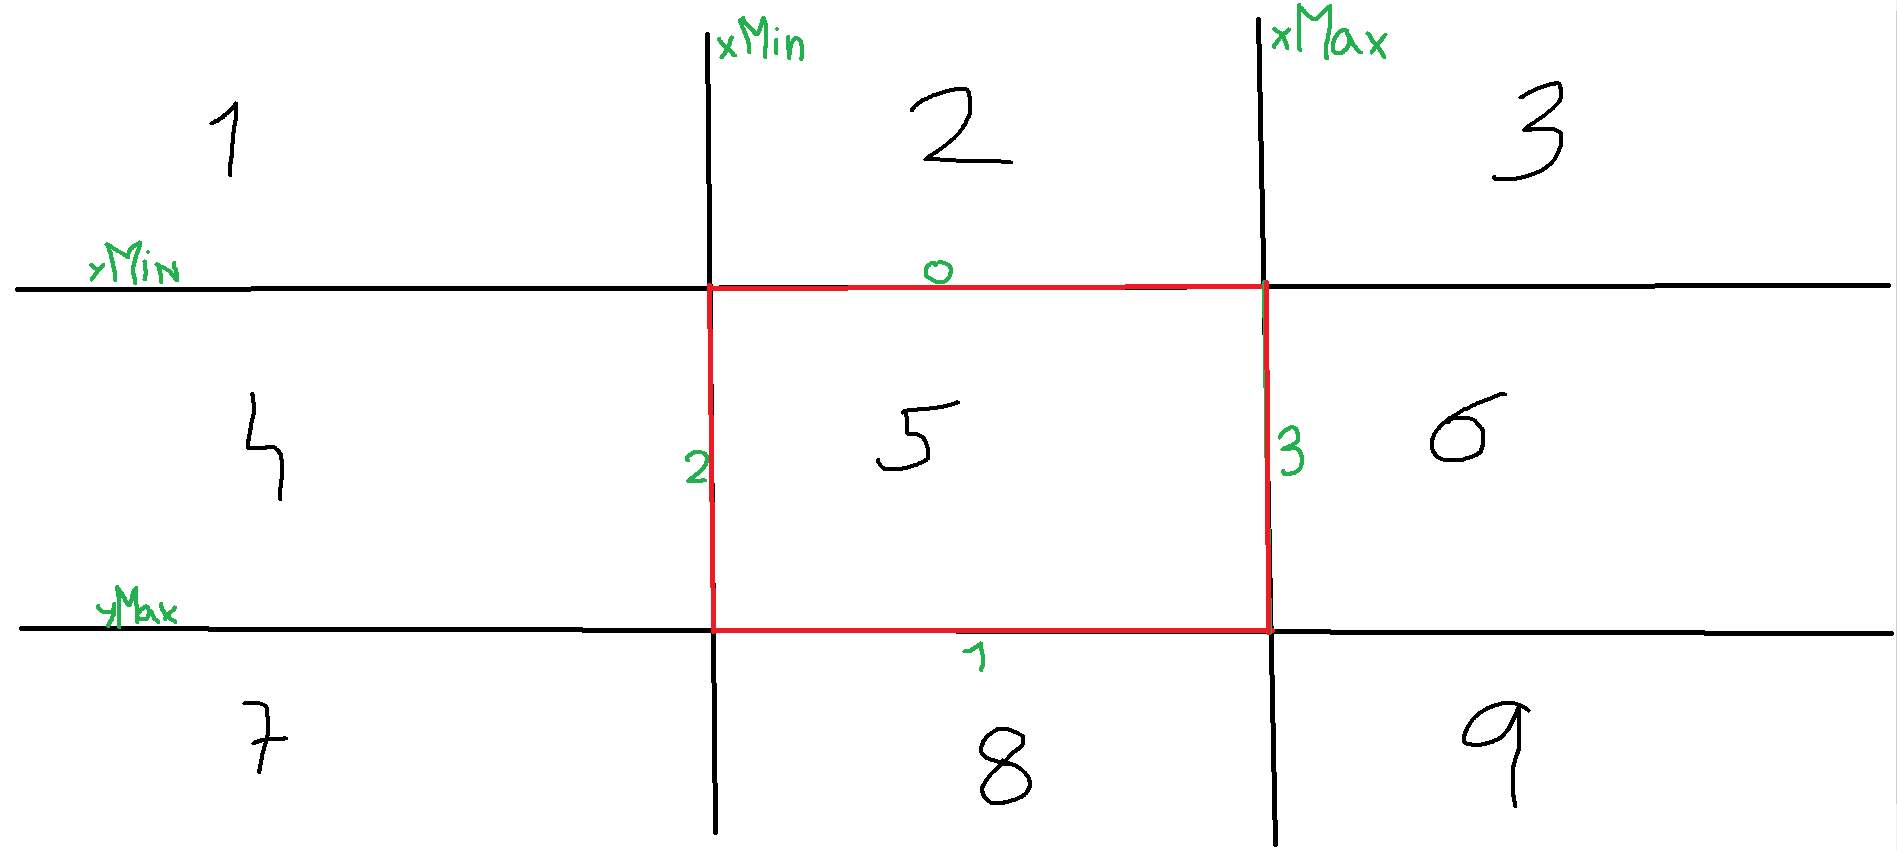
\includegraphics[width=0.7\linewidth]{Obrazky/Schema mistnosti.png}
    \caption{Schéma místností Zdroj: vlastní}
    \label{fig:enter-label}
\end{figure}


\subsubsection{Odstraňování}
Vlna se odstraní pokud je její amplituda menší než nula nebo je starší než \textit{maxAge} (8 sekund). \textit{maxAge} byl zvolen jako 8 sekund, protože tolik trvá \textit{innerCircle},  než se expanduje pryč z místnosti.

\subsubsection{Odraz}
Zvuková vlna se odrazí, pokud se dotkne stěny. Tato logika v programu funguje následovně. Nejprve se zjistí, při jakých poloměrech se vlna odrazí od zdi, neboli jak moc je vlna vzdálená od každé zdi. Tyto vzdálenosti najde metoda \textit{getReflectionDistances}, která vrací pole celých čísel / integerů. Nejdříve metoda zjistí v jakém sektoru scény (viz. obrázek 5) leží pomyslný střed (v případě kdy je vlna vytvořena kliknutím uživatele, tak reálný střed). Vlna se může nacházet v devíti různých sektorech 1-9, které tvoří 3 logicky podobné skupiny (první je 5, druhá je 2,4,6,8 a třetí je 1,3,7,9). Skupiny jsou si podobné tehdy když mají osy vlny v daných skupinách stejný počet průsečíku se stěnami místnosti. Pro první skupinu jsou průsečíky 4, pro druhou je jeden a pro třetí je jich 0.
To, jestli střed leží v daném sektoru, zjišťují metody: \textit{isInRectangle, isBellowRectangle,isAboveRectangle, isLeftOfRectangle, isRightOfRectangle, isAboveOnTheRightOfRectangle, isAboveOnTheLeftOfRectangle, isBellowOnTheRightOfRectangle, isBellowOnTheLeftOfRectangle}. Tyto metody vrací boolean a jsou použity jako podmínky v if-else if řetězci v metodě \textit{getReflectionDistances}.\\
Jako první a nejjednodušší na počítání je sektor 5, střed vlny je reálný a nachází se v místnosti. Vzdálenosti se tehdy určují pouze jako vzdálenosti průsečíků os se stěnami a středem. Tyto vzdálenosti jsou 4 tím pádem metoda vrátí pole integeru o velikosti 4. Dále s těmito vzdálenostmi pracuje třída \textit{WaveManager}.\\
Pro druhou skupinu neboli sektory 4,8,6,8 se ve třídě \textit{SoundWave} počítá pouze jedna vzdálenost a to ta od středu k průsečíku opačné strany. V tomto případě metoda vrací pole o velikosti 1 s danou vzdáleností, ostatní vzdálenosti počítá třída \textit{WaveManager}.\\
Třetí skupina se počítá jinak než první 2. Jelikož je střed vlny diagonálně od místnosti, tak osy vlny nemají se stěnami místnosti žádný průsečík, proto je zde potřeba uplatnit jiný výpočet odrazových vzdáleností. Protože se vlna šíří jakoby z rohu místnosti, tak se vždy dotkne první rohů opačných stěn. Takže je nutné vypočítat pouze vzdálenosti k ostatním rohům místnosti. Počet těchto vzdáleností je 3 takže metoda vrací pole o velikosti 3. 

\subsubsection{Vykreslování}
Zvuková vlna má tvar donutu, tento tvar program chápe jako prostor mezi vnějším (\textit{ounterCircle}) a vnitřním kruhem (\textit{innterCircle}). Prostor je rozdělen na 20 ( včetně \textit{innerCircle} a \textit{outerCircle}) podkružnic. Počet těchto podkružnic je roven podílu velikosti pixelu (\textit{PIXELSIZE}) a vlnové délky / rozdílu poloměru vnějšího a vnitřního kruhu (\textit{deltaR}). \\
Každá z těchto podkružnic zvýší nebo sníží celkovou výchylku daného pixelu o \textit{amplituda/5}. Prvních 5 ji zvýší, druhých 10 ji sníží a zbytek ji zvýší. Toto vytvoří iluzi sinusoidy s jednoduchou a velmi efektivní implementací v kódu. Konkrétně to funguje následovně.\\ 
Pokaždé když se zavolá metoda \textit{grow()} a \textit{outerRadius} je dělitelný \textit{PIXELSIZE}, tak se volá metoda \textit{generateWaveDonut()}. Tato metoda nejprve vypočítá aktuální délku vlny (\textit{width}) a potom vypočítá celkový počet kruhů (\textit{numberOfCircles}), ten se spočítá jako podíl délky vlny a \textit{PIXELSIZE}. Následovně je spuštěn for-cylkus, který běží od nuly do \textit{numberOfCircles}. V tomto for-cyklu se nejprve vypočítá poloměr momentální podkružnice,
\begin{minted}{java}
int radius = innerRadius + ((numberOfCircles - i-1) * PIXELSIZE)
\end{minted}
potom její okamzitaVychylka (\textit{amplitudeForCirrcle}) pomocí metody \textit{calculateAmplitudeForCircle(int circleIndex)}. Tato metoda vrátí buď \textit{amplitude/5}, pokud je index menší než 5 nebo větší než 15, nebo 
\textit{-amplitude/5,} pokud je hodnota indexu jiná. \\
Dále se zavolá metoda \textit{drawCircleWithOkamzitaVychylka(int centerX, int centerY, int radius, int okamzitaVychylkaValue)}\cite{algoritmus}. Tato metoda použije Bresenhamův algoritmus na vykreslování kružnic a zjistí na jakých pixelech (reálné celočíselné pixely na obrazovce) momentálně kružnice leží. 
\begin{minted}{java}
    int x = 0;
    int y = radius;
    int d = 3 - 2 * radius;
    //finds the coordinates of pixels
    while (y >= x) {
        if (d > 0) {
            y--;
            d = d + 4 * (x - y) + 10;
        } else {
            d = d + 4 * x + 6;
        }
        // Set the pixels for this circle
        setCirclePixelsDisplacement
        (centerX, centerY, x, y, okamzitaVychylkaValue);
        x++;
    }
\end{minted}
Hodnoty jsou předány metodě \textit{setCirclePixelsDisplacement(int centerX, int centerY, int x, int y, int okamzitaVychylkaValue)}, která zjistí zda je daná souřadnice v místnosti. Jelikož Bersenhamův algoritmus funguje na bázi kopírování pixelů symetricky podle středu a os symetrií, tak je potřeba zjistit zda se daný pixel nachází v místnosti. To metoda rozpozná za pomoci 8 podmínek (8 protože kruh je symetrický po 8 osách). Zde je příklad několika z těchto podmínek. 
\begin{minted}{java}
if (centerY + y > yMin && centerY + y < yMax &&
    centerX + x > xMin && centerX + x < xMax)
if (centerY + y > yMin && centerY + y < yMax &&
    centerX - x > xMin && centerX - x < xMax)
if (centerY - y > yMin && centerY - y < yMax &&
    centerX + x > xMin && centerX + x < xMax)
if (centerY - y > yMin && centerY - y < yMax &&
    centerX - x > xMin && centerX - x < xMax)
\end{minted}
Pokud se tyto podmínky splní, tak se zavolá metoda setPixelDisplacement(int x, int y, int okamzitaVychylkaValue), jenž přidá okamžitou výchylku kruhu na jednotlivé pixely. Jako první se konvertují souřadnice na scéně na souřadnice v \textit{pixelGridu} pomocí metody \textit{getGridX/Y} ze třídy Pixel. Dále se zkontroluje, zda jsou gridové souřadnice validní a pokud jsou, tak se vytvoří nová instance třídy \textit{PixelCoordinate} \textit{ pixelCoord} se souřadnicemi \textit{gridX/Y}. Poté se zkontroluje, zda daný \textit{pixelCoord} nebyl už jednou přidaný, to znamená jestli není v setu \textit{visitedPixels}. Pokud je tak se přidá do setu \textit{duplicatePixels}, a pokud není, tak se přidá do setů \textit{visitedPixels} a \textit{activePixelCoordinates}, a  \textit{Pixelu} se stejnými souřadnicemi v \textit{pixelGridu} se přidá \textit{okamzitaVychylka} kružnice.  


